
\documentclass[a4paper, nobib]{tufte-handout}
%%%%%%%%%%%%%%
%  Packages  %
%%%%%%%%%%%%%%
\usepackage{pgfplots}
\pgfplotsset{compat=1.16}
\usepackage{tikz}
\usepackage{subfig}
\usepackage{hyperref}
\usepackage{minted}
\usepackage[utf8]{inputenc}
\usepackage[T1]{fontenc}
\usepackage{amsmath}
\usepackage{natbib}
\usepackage{booktabs}
\usepackage[inline]{enumitem}
\usepackage{array}
\usepackage{multicol}
\usetikzlibrary{matrix}
\usepackage{algorithmic}
\definecolor{lightBlue}{RGB}{180,40,188}
\definecolor{sexyRed}{RGB}{175,30,45}
\definecolor{sexyBlack}{RGB}{52,52,52}
\hypersetup{
    pdffitwindow=false,            % window fit to page
    pdfstartview={Fit},            % fits width of page to window
    pdftitle={Lab notes 2014},     % document title
    pdfauthor={Your Name},         % author name
    pdfsubject={},                 % document topic(s)
    pdfnewwindow=true,             % links in new window
    colorlinks=true,               % coloured links, not boxed
    linkcolor=sexyRed,      % colour of internal links
    citecolor=lightBlue,       % colour of links to bibliography
    filecolor=sexyBlack,            % colour of file links
    urlcolor=lightBlue           % colour of external links
}


%%%%%%%%%%%%%%%
%  meta data  %
%%%%%%%%%%%%%%%
\title{Assignment 2}
\newcommand{\institution}{Ecole Nationale Supérieure d'Arts et Métiers}
\date{22 February 2020}

\begin{document}
\maketitle
%{{{Seam Carving
\section{Seam Carving (5 points)}

The goal of this assignment is to implement from  \emph{scatch} the \textbf{Seam
Carving} method.\\[4pt]

\textbf{Resources}:\\
%{{{
\begin{itemize}
  \item Paper on seam carving 
    \href{http://graphics.cs.cmu.edu/courses/15-463/2007_fall/hw/proj2/imret.pdf}{Seam
  Carving} paper.
\item Tutorial \href{http://cs.brown.edu/courses/cs129/results/proj3/taox}{Brown
  university}
\item Tutorial 2 \href{http://www.cs.cmu.edu/afs/andrew/scs/cs/15-463/f07/proj2/www/wwedler/}{Andrew
blog}
\end{itemize}
%}}}
\begin{enumerate}
  %{{{ Magnitude of gradient
  \item \textbf{Compute the magnitude of image gradients.}\\
    We will not only compute the gradients but also the energy function in
    each pixel of the image.
    %{{{ Code
      \begin{minted}[frame=lines, fontsize=\scriptsize]{python}

def energy_function(image):
    """Computes energy of the input image.

    Args:
        image: numpy array of shape (H, W, 3)

    Returns:
        out: numpy array of shape (H, W)
    """
    H, W, _ = image.shape
    out = np.zeros((H, W))

    # convert the image to grayscale
    image = color.rgb2gray(image)
    
    #computing the gradient
    Gx, Gy = np.gradient(image)

    #taking the L1 norme
    out = np.abs(Gx) + np.abs(Gy)

    return out
      \end{minted}
    %}}}

%{{{Images 
\begin{marginfigure}
  \centering
  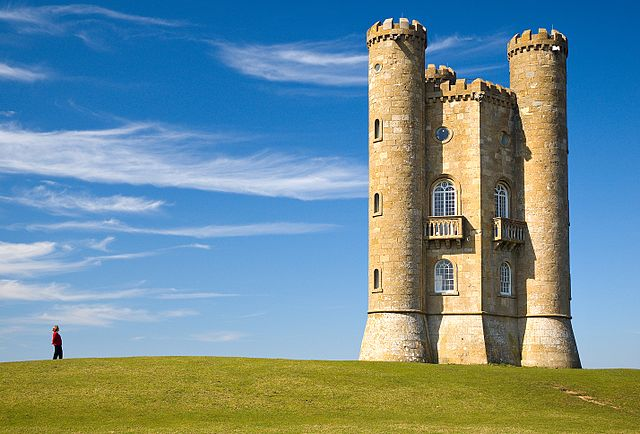
\includegraphics[width=6cm, height=4cm]{imgs/broadway_tower.jpg}
  \caption{Initial Image}
\end{marginfigure}

\begin{marginfigure}
  \centering
  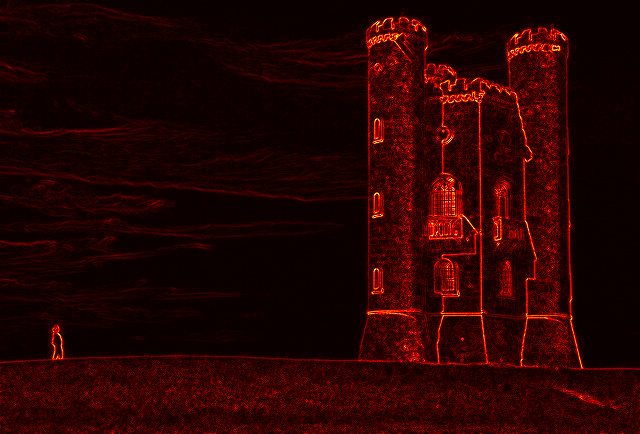
\includegraphics[width=6cm, height=4cm]{./broad_way_energy.png}
  \caption{Energy}
\end{marginfigure}
%}}}
  %}}}
%{{{Path with the smallest energy
\item \textbf{Find the path with the smallest energy}

  \begin{itemize}
    \item \textbf{Compute the cost on each point}: Once we computed the energy,
      We will compute the cost for each pixel. The procedure starts from the
      first line and uses \emph{dynamic programming} to compute the minimal cost
      from the parents. the code is in the function
      \mintinline{python}{compute_costs(I, energy)} in the
      \texttt{seamcarving.py} file. The function also returns a \texttt{Path}
      which indicate the parent for each pixel in order to compute the seam.
      
      In the \autoref{fig:costs}, we show the vertical and horizontals seams.
      The figure clearly show that costs are higher near the tower.

    \item \textbf{Finding Optimal Seams:}  Using the cost we computed in
      previous item, We could compute the seam with the lowest energy in the
      Image. Then, we could remove seam by seam until we attain the desired
      \textbf{width} or \textbf{height}

      \begin{itemize}
        \item First, the function \mintinline{python}{backtrack_seam(paths, end)} where \texttt{end} is the pixel with the lowest cost. Either in
          the last row or column depending the reducing mode. The function
          simply track the parents to find the seam.
        \item Second, we apply  the function \mintinline{python}{remove_seam(Img,
          seam)} to remove the seam from the Image.

        \item This function \texttt{remove\_seam} is repeated until get get the
          desired Size. 
      \end{itemize}
      In the \autoref{fig:seam_reduction}, we show the resized Image after seam
      remove in both directions.
  \end{itemize}


  \begin{figure}[ht!]
  \subfloat[a][Vertical]{
  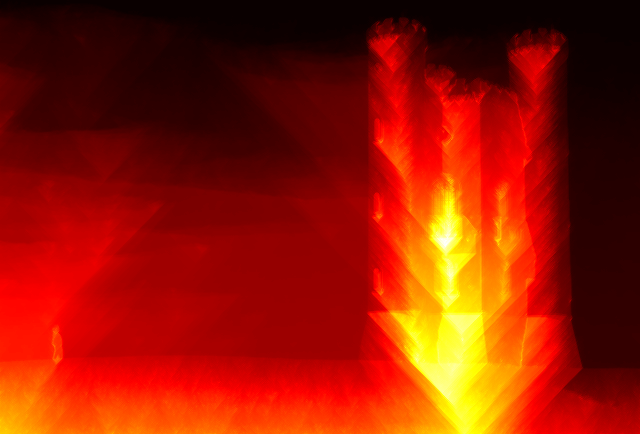
\includegraphics[width=5cm, height=4cm]{./v_costs.png}
}
\hfill
  \subfloat[b][Horizontal]{
  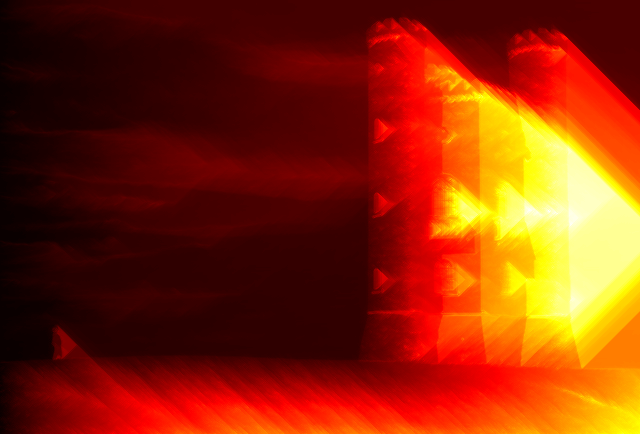
\includegraphics[width=5cm, height=4cm]{./h_costs.png}
}
\caption{Vertical and Horizontal cost  functions}
\label{fig:costs}
\end{figure}

Here is the figure showing the backtracked seam. The seam is traced with the red
color.

\begin{figure}[htpb]
  \centering
  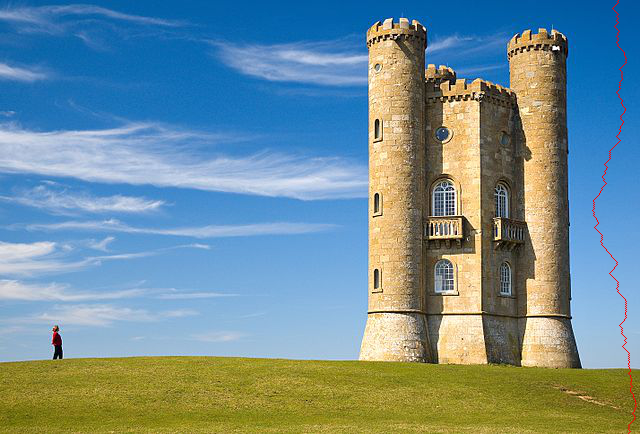
\includegraphics[width=0.8\linewidth,height=5cm]{"./vseam.png"}
  \caption{Vertical Minimal Seam}%
  \label{fig:v_seam}
\end{figure}


\begin{figure}[htpb]
  \centering
  \subfloat[][initiale]{
  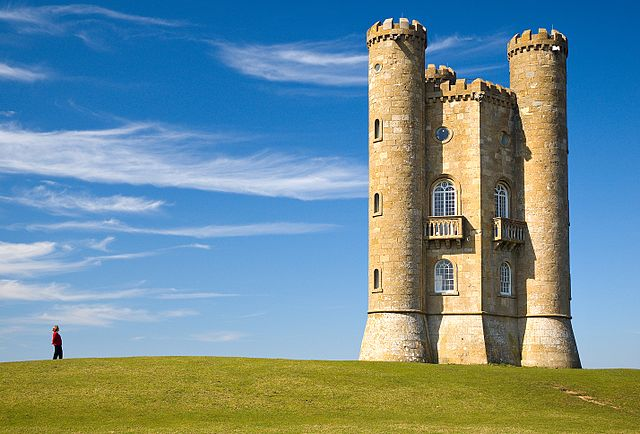
\includegraphics[width=5cm, height=4cm]{imgs/broadway_tower.jpg}
}
\hfill
  \subfloat[][reduced]{
  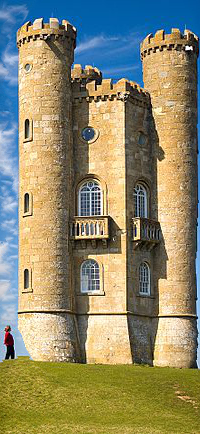
\includegraphics[width=2.5cm,height= 4cm]{./reduced.png}
}
  \caption{Reduced Image}%
  \label{fig:seam_reduction}
\end{figure}

%}}}

\end{enumerate}
%}}}
%{{{ KeyPoint Detection
\section{KeyPoint Detection}%
\label{sec:keypoint_detection}

\begin{enumerate}
  \item \textbf{Implement a function to perform \textbf{Harris corner}
    detection?}
  %{{{ Harris Corner code
      \begin{minted}[frame=lines, fontsize=\scriptsize]{python}

def harris_corners(img, window_size=3, k=0.04):
    """
    Compute Harris corner response map. Follow the math equation
    R=Det(M)-k(Trace(M)^2).
        
    Args:
        img: Grayscale image of shape (H, W)
        window_size: size of the window function
        k: sensitivity parameter

    Returns:
        response: Harris response image of shape (H, W)
    """

    H, W = img.shape
    window = np.ones((window_size, window_size))

    response = np.zeros((H, W))

    dx = filters.sobel_v(img)
    dy = filters.sobel_h(img)

    #convolving 
    dxc = convolve(dx**2, window)
    dyc = convolve(dy**2, window)
    dxcc= convolve(dx*dy, window) 
    #creating the main matrix
    M= np.zeros((2*H, 2*W))
    
    #storing the main matrix
    M[::2,::2] = dxc
    M[1::2,1::2] = dyc
    M[::2,1::2] = dxcc 
    M[1::2,::2] = dxcc
    
    M= view_as_blocks(M, block_shape=(2,2))

    for i in range(H):
        for j in range(W):
            mat = M[i,j]
            lam,eigenVec =np.linalg.eig(mat)
            response[i,j] = lam.prod()- k*(lam.sum()**2)

    return response

    \end{minted}
    %}}}
%{{{Figure
  \begin{figure}[ht!]
  \centering
  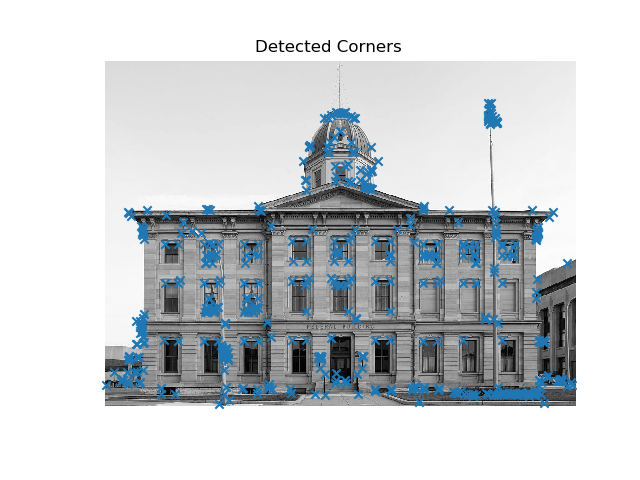
\includegraphics[width=10cm, height=5cm]{./harris_response.png}
\end{figure}
%}}}

%{{{Lowe's SIFT Descriptor
\item \textbf{Implement Lowe's Scale invariant interest point detection. Let the
  number of scales per octave be a parameter of your code?}
%}}}
\end{enumerate}

%}}}

\end{document}
